\documentclass{article}


\usepackage{arxiv}

\usepackage[utf8]{inputenc} % allow utf-8 input
\usepackage[T1]{fontenc}    % use 8-bit T1 fonts
\usepackage{hyperref}       % hyperlinks
\usepackage{url}            % simple URL typesetting
\usepackage{booktabs}       % professional-quality tables
\usepackage{amsfonts}       % blackboard math symbols
\usepackage{nicefrac}       % compact symbols for 1/2, etc.
\usepackage{microtype}      % microtypography
\usepackage{lipsum}
\usepackage{etoolbox}
\usepackage{amsmath}
\usepackage{subcaption}
\usepackage{graphicx}

\graphicspath{{images/}}
\captionsetup[figure]{labelfont={large},textfont={large}}
\captionsetup[subfigure]{labelfont={}, textfont={}}

\title{Automated Market Making}


\author{
  Chris Slaughter and Brandon Eng \\
  Level\\
  Los Angeles, CA 90004 \\
  \texttt{\{chris, brandon\}@lvl.co}
}

\begin{document}
\maketitle

\begin{abstract}

The role of a market maker is to provide liquidity on an exchange by quoting bid and ask prices for a small discount or premium to the market price. Automated market making is an active strategy that continuously makes the market in one or more assets. Automated market making has been extensively studied, and an optimal market making algorithm has been proposed by Avellaneda \& Stoikov (2008). In this paper, we review the state of the art in optimal market making, and then propose a simplified market making model that relies on only two parameters: spread and give. We also demonstrate the performance of the model in simulations.

\end{abstract}

\keywords{Exchange \and Liquidity \and Automated Market Making}

\section{Introduction}
\label{sec:intro}

Market makers create liquidity on a market by quoting bid and ask prices for a trading asset near the market price. Market makers profit by quoting asks at a premium, and bids at a discount, to the market price. This premium or discount is referred to as the market maker \emph{spread}. Market makers realize the spread each time an order is matched at their quoted price. The \emph{arrival rate} of orders is lower for market makers that charge high spreads, and both spread and arrival rate must be balanced for a market maker to maximize profit. The market maker must also manage the \emph{inventory} of cash and asset available to fulfill market demand, as well as the opportunity cost of taking a net long position in inventory. In all, the market maker must consider:

\begin{itemize}
	\item The spread charged
	\item The arrival rate of orders
	\item Available inventory of cash and asset
	\item Opportunity cost of holding inventory
\end{itemize}

While profitable market making is a complex and multidimensional problem, it has also been extensively studied in the literature, particularly in two seminal papers. Ho \& Stoll studied the problem of dealing under competition and found that the bid and ask quotes are related to the reservation (or indifference) price of the dealer \cite{ho1980on}. Then Avellaneda \& Stoikov proposed a model combining the utility formulation of Ho \& Stoll with statistical modeling of the microstructure of a limit order market, and solved optimal market pricing under this model \cite{avellaneda2008high}. The solution of Avellaneda \& Stoikov is notable because it demonstrates a stochastic optimal control policy under a reasonable stochastic model for order arrivals \cite{bouchard2002statistical}. Subsequent work by Guéant, Lehalle, \& Tapia extended this solution to consider management of a finite inventory of cash and asset \cite{guéant2012dealing}. In Section \ref{sec:optimal}, we review the state of the art algorithms for market making to provide context for our algorithm.

In the first paragraph of their seminal 2008 paper, Avellaneda \& Stoikov noted of market making:

\begin{quote}
Traditionally, this role has been filled by market maker or specialist firms. In recent years, with the growth of electronic exchanges such as Nasdaq’s Inet, anyone willing to submit limit orders in the system can effectively play the role of a dealer. Indeed, the availability of high frequency data on the limit order book (see www.inetats.com) ensures a fair playing field where various agents can post limit orders at the prices they choose.
\end{quote}

While in principle, anyone may play the role of market maker in a market, various limitations prevent this in practice. US securities law limits who may make the market based on accreditation rules, brokerage licensing requirements, and other considerations. In commodities markets including cryptocurrency spot markets, the high technical complexity of market making 24/7 as well as fee discounts offered to incumbents create competitive barriers to entry for retail participants. While the barriers to entry for automated market making remain high, automation technology has made other active strategies such as market-weighted rebalancing and tax-loss harvesting widely avaiable to retail customers in products such as Wealthfront and Betterment \cite{wealthfront, betterment}.

In using automation to provide retail access to active strategies, particular attention must be paid to both \emph{algorithm design} and \emph{interface design}. Making investment decisions is proven to be complex. Monti, Martignon, Gigerenzer, \& Berg studied high-stakes financial decisions made by bank customers and found that investors cling to the information available to them, ignoring more complex variables which are often assumed in economic models \cite{monti2009impact}. To prevent the end user from adversely selecting a non-competitive policy configuration, we call for making the policy configuration human readable and educating investors on the underlying dynamics of their decisions. Our objective is to devise an automated strategy for continuous market making that considers the traditional utility objectives of market making, as well as the usability objectives of making market making broadly available to retail users for the first time. In total, the considerations include:

\begin{itemize}
  \item The spread charged
  \item The arrival rate of orders
  \item Available inventory of cash and asset
  \item Opportunity cost of holding inventory
  \item Practical deployment across user accounts
  \item Intuitive policy configuration
\end{itemize}

In Section \ref{sec:optimal} we review the state of the art algorithms for optimal market making. In Section \ref{sec:retail} we propose an algorithm that reflects the structure of optimal market making, while simplifying parameterization of the algorithm to promote optimal policy configuration. In Section \ref{sec:experiments} we demonstrate the performance of this algorithm in simulation.

\section{Optimal Market Making}
\label{sec:optimal}

In this section, we re-summarize the model of Avellaneda \& Stoikov based on the notation and summary of Guéant, Lehalle, \& Tapia. We refer to this model herein as the \emph{standard model}.

In the standard model, the market price, which may be the market mid-price or a reference quote, moves as arithmetic Brownian motion:

\begin{equation}
\label{eq:brownian}
dS_{t} = \sigma dW_{t}
\end{equation}

Guéant, Lehalle, \& Tapia note in a footnote that Equation \ref{eq:brownian} is almost equivalent to the standard Black-Scholes model on a short time horizon, i.e. in a narrow time window the price is exclusively affected by random, drift-free arrival of the arrival of order matches on the limit order market. The market making agent continuously quotes bid and ask prices, $S^b_t$ and $S^a_t$ respectively, and will therefore buy and sell shares of the asset based on the random arrival of orders matched at the quoted prices. In the standard model, the agent holds accumulative inventory $q_t$ given by:

\begin{equation}
\label{eq:inventory}
q_{t} = N^b_{t} - N^a_{t}
\end{equation}

where $N^b_{t}$ and $N^a_{t}$ are the point processes representing the number of asset bought bought or sold respectively as order matches arrive at the quoted prices. The standard model assumes that the intensity of arrival of order matches decreases monotonically in the spread offered on the quoted price. Assuming a bid spread of $\delta^b_t = S_t - S^b_t$ and an ask spread of $\delta^a_t = S^a_t - S_t$, the intensity of arrivals for bids and asks, $\lambda^b$ and $\lambda^a$ respectively, are given by:

\begin{equation}
\label{eq:arrival}
\lambda^b = A \exp^{-k \delta^b_t}, \quad
\lambda^a = A \exp^{-k \delta^a_t}
\end{equation}

where $A$ and $k$ are positive constants characterizing the liquidity of the asset. Modeling the arrival of order matches permits the agent's net cash holdings to be characterized as well by:

\begin{equation}
\label{eq:cash}
dX_t = ( S_t + \delta^a_t ) dN^a_t - ( S_t - \delta^a_t ) dN^b_t
\end{equation}

A notable contribution of Guéant, Lehalle, \& Tapia is the introduction of an inventory bound $Q$. The inventory held by the agent, $q_t$, which is signed in the standard model, is bounded in the interval $|q_t| < Q$. Put differently, the agent may never hold more than $Q$ asset, and the agent may never go net short $Q$. While this constraint imposes a realistic risk limit, it does not lead immediately to a risk-based \emph{inventory policy}. For example, the standard model does not model the agent's starting inventory. We address these practical limitations in Section \ref{sec:retail}.

The standard model culminates in the proposal of a utility function which is maximized by the optimal control policy $(\delta^b_t, \delta^a_t)_t$. The utility function and control policy are given by:

\begin{equation}
\label{eq:utility}
\max_{(\delta^b_t, \delta^a_t)_t \in \mathcal{A}} \mathop{\mathbb{E}} [ - \exp(-\gamma(X_T + q_T S_T)) ]
\end{equation}

where $T$ is the terminal time, $\mathcal{A}$ is the set of predictable policies and $\gamma$ is the agent's risk aversion coefficient. Note that $X_T + q_T S_T$ is the value of the portfolio at time $T$, which is directly proportional to agent P\&L, and that $f(x) = \exp(-\gamma x)$ is monotonic in $x$. As a result, the stochastic optimal control objective can be seen as related to maximizing agent P\&L.

The canonical solution to this problem, provided by Avellaneda \& Stoikov, is given by the following quoting policy:

\begin{equation}
\label{eq:avellanedastoikov1}
r_t(s) = s - q \gamma \sigma^2(T - t)
\end{equation}

\begin{equation}
\label{eq:avellanedastoikov2}
\delta^a_t + \delta^b_t = \gamma \sigma^2(T - t) + \frac{2}{\gamma}(1 + \frac{\gamma}{k})
\end{equation}

Here, $r_t(s)$ is the reservation price of the agent, and $\delta^a_t + \delta^b_t$ is the spread. We can make several intuitive observations about the optimal policy. The reservation price is the market reference price, adjusted by a give of $q \gamma \sigma^2(T - t)$. We refer to this as a give because it manifests as a discount to the ask quote when the agent is overweight and a premium to the bid quote when the agent is overweight, both of which give advantage to the taker relative to the reference price $s$. The give is linear in inventory $q$, proportional to volatility $\sigma^2$, and straightlines to zero as the trading interval elapses. The spread $\delta^a_t + \delta^b_t$ follows a similar formula, but does not rely on inventory, and straightlines to the constant $\frac{2}{\gamma}(1 + \frac{\gamma}{k})$ as the trading interval elapses. 

In summary, the optimal control policy charges a spread independent of inventory against a price adjusted to manage inventory. In the next section we simplify the structure of these equations to arrive at a policy in terms of spread and give.

\section{Retail Market Making}
\label{sec:retail}

In this section, we propose a policy for market making that reflects the dynamics of the policies discussed in Section \ref{sec:optimal}, but that is also formulated to be easily configured by a casual user. Designing simple-to-use configuration interfaces for automated strategies mitigates adverse selection risk and maintains efficient market operation in a market where potentially most agents operate identical policies (up to configuration).

Our policy replaces the spread Equation \ref{eq:avellanedastoikov2} with a user specified percentage spread $\Delta$, resulting in the overall spread:

\begin{equation}
\label{eq:retailspread}
\delta^a_t + \delta^b_t = 2 \Delta s
\end{equation}

We believe a user's selection of $\Delta$ encapsulates their thinking about arrival rate $k$ and risk coefficient $\gamma$ without requiring education on either auxiliary variable. For example, a user will choose a lower spread to encourage faster order arrivals. The spread is clearly no longer a linear form, or even a function of, volatility $\sigma$. We believe this is justified because the user thesis on market volatility is also captured by their selection of spread, since overwide spreads will not experience order arrivals. By wholely substituting spread with a user-specified quantity, our algorithm does not impose an automatic policy for spreads but rather requires the user to configure spread \emph{as policy}. We believe this decision is justified since any marginal decision to expand the complexity of Equation \ref{eq:retailspread} introduces advanced market concepts to the interface, while eroding understanding of what net spread the agent charges the market for its services.

Our policy restates the user reservation price in terms of \emph{reference price} and \emph{give}. To arrive there constructively, recall the formulation of reservation price from Section \ref{sec:optimal}, $r_t(s) = s - q \gamma \sigma^2(T - t)$. By performing the change of variables $q \mapsto q/Q = q'$, we arrive at the alternative formulation:

\begin{equation}
\label{eq:retailprice}
r_t(s) = s - q' Q \gamma \sigma^2(T - t) = s - q' G'
\end{equation}

We recall the inventory risk constraint $|q| < Q$ and note that if it was enforced by the agent, then $|q'| < 1$ achieving the limits $q = -1$ when the agent is totally underweight the asset and $q = 1$ when the agent is totally overweight the asset. Therefore $G'$ may be interpreted as the maximum give on price the agent will provide to rebalance inventory. Performing the additional change of variables $G' \mapsto G'/s = G$, the equation can be written as:

\begin{equation}
\label{eq:retailpricepercentage}
r_t(s) = s - q' G s = s (1 - q' G)
\end{equation}

Here, $G$ is the maximum give as a percentage of asset price. This modification normalizes the specification of give for any market price. We believe the most intuitive experience for the user is to specify the give outright, since the give is a percentage like spread, characterizes the loss in profit offered to rebalance explicitly, and encapsulates user thinking on volatility and risk.

The quote pricing in our policy is then given as:

\begin{equation}
\label{eq:retailbid}
s^b_t = s_t (1 - q_t' G - \Delta)
\end{equation}
\begin{equation}
\label{eq:retailask}
s^a_t = s_t (1 - q_t' G + \Delta)
\end{equation}
\begin{equation}
\label{eq:retailqprime}
q_t' = \frac{s_t q_t - x_t}{s_t q_t + x_t}
\end{equation}

This policy quotes a spread that is constant in inventory and a reservation price that is linear in inventory, which we believe to be the most important dynamics of the linear stochastic control policy. However the simplification of the policy configurations as $(\Delta, G)$ reduces the risk of adverse selection of noncompetitive policy configurations.

While the policy reflects inverse linear control of reservation price like the optimal policy, we make no claim that the modified policy is optimal in any sense. We believe that it provides only an engineered compromise between optimal policy, ease of configuration, and practical considerations such as finite, non-negative inventory.

\section{Experiments}
\label{sec:experiments}

There have been numerous recent numerical reproductions of the results of Avellaneda \& Stoikov \cite{fushimi2018optimal} as well as commercial deployments of the algorithm. In this Section, we simulate our algorithm 

\begin{figure}[t!]

\begin{subfigure}{0.49\textwidth}
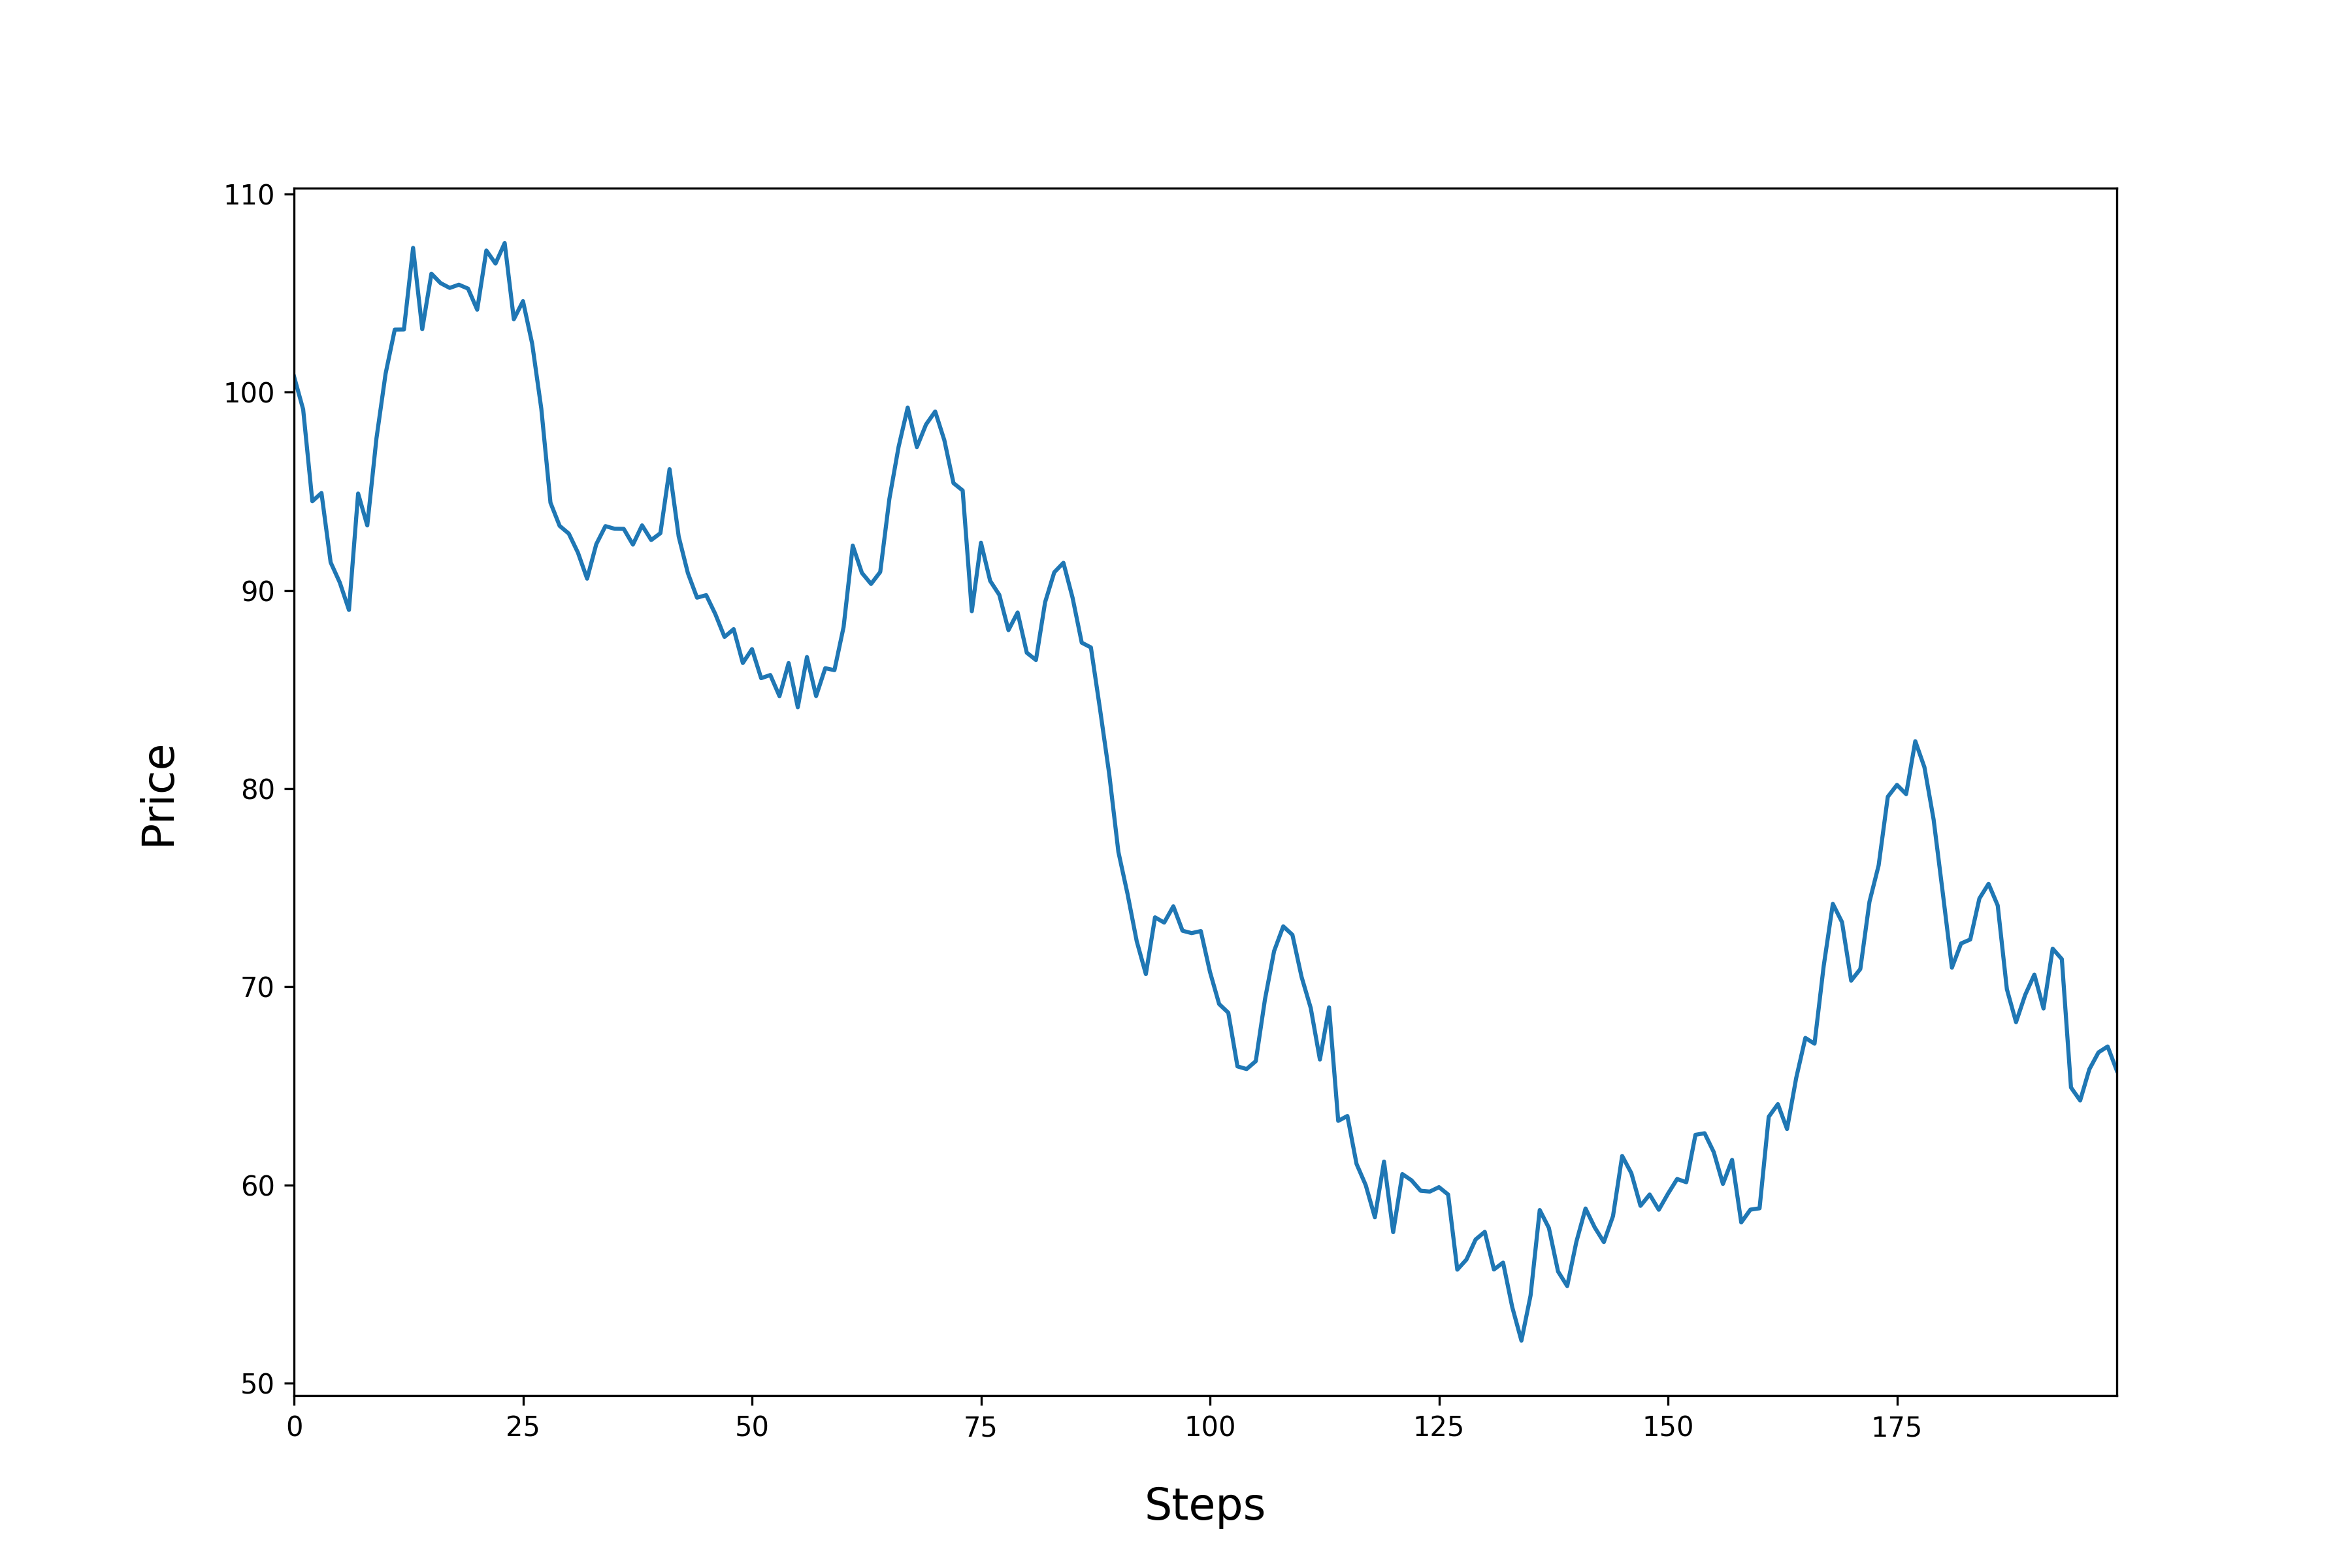
\includegraphics[width=\linewidth]{test.png}
\caption{First subfigure} \label{fig:a}
\end{subfigure}\hspace*{\fill}
\begin{subfigure}{0.5\textwidth}
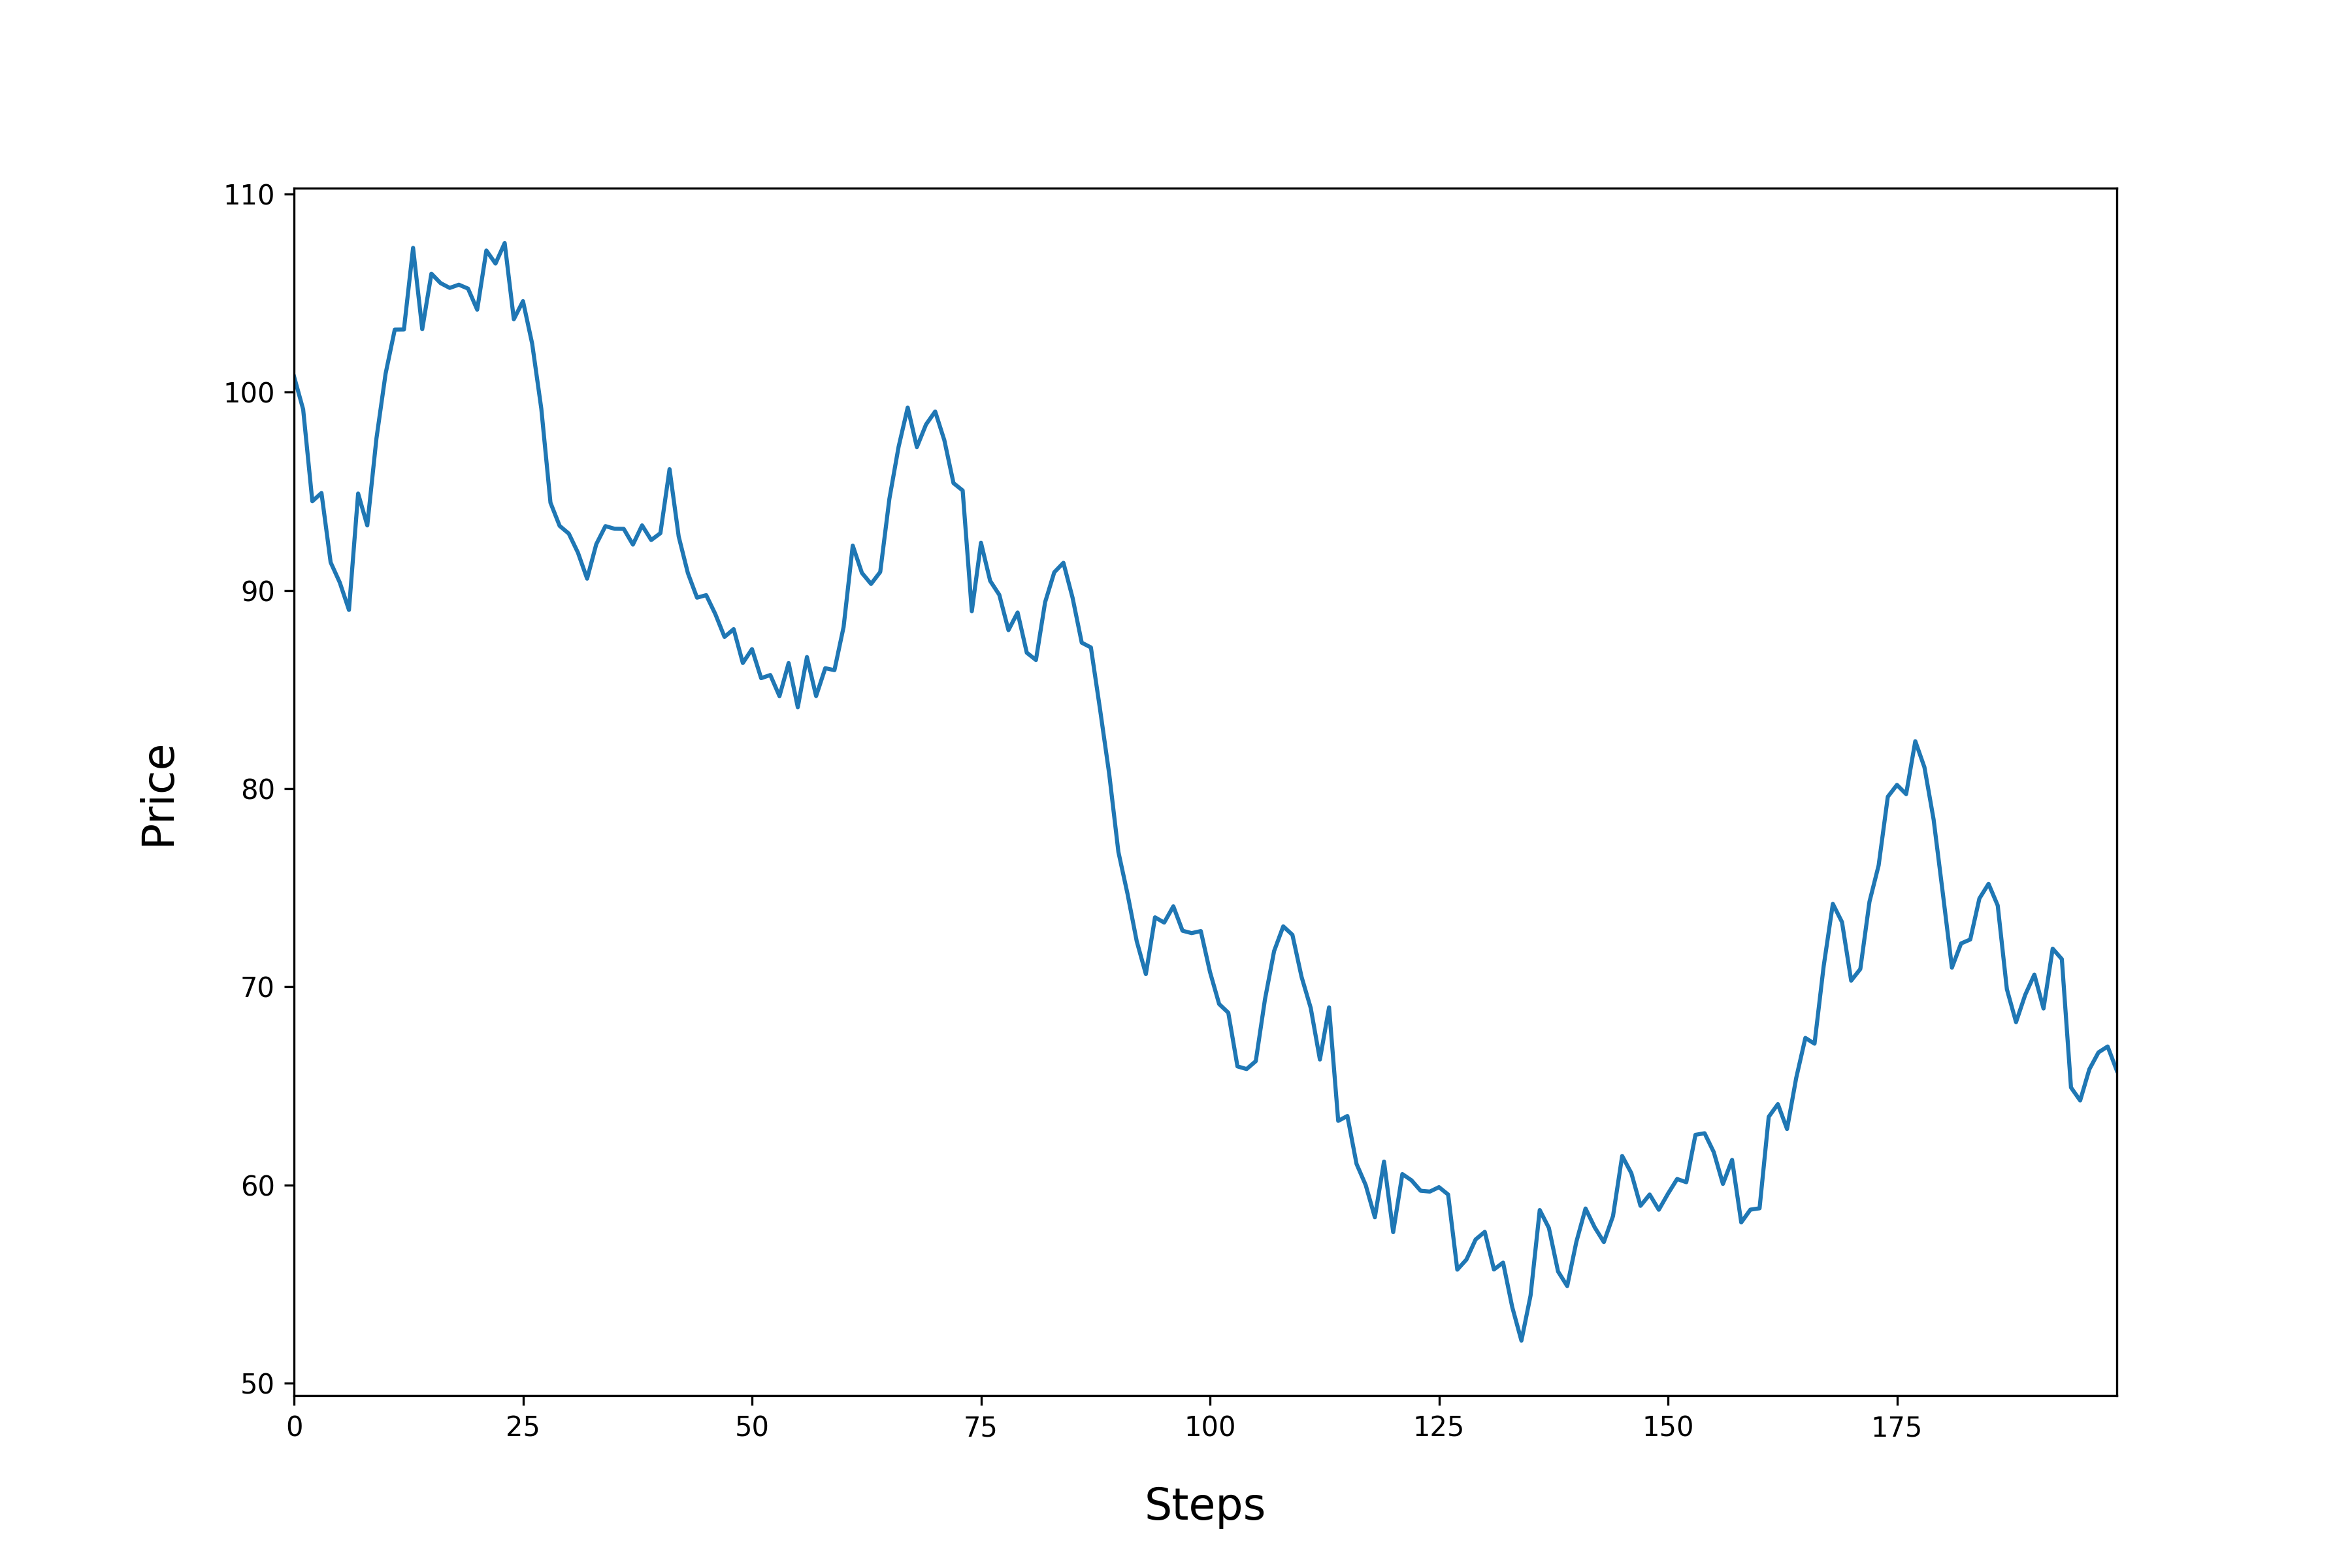
\includegraphics[width=\linewidth]{test.png}
\caption{Second subfigure} \label{fig:b}
\end{subfigure}

\medskip
\begin{subfigure}{0.49\textwidth}
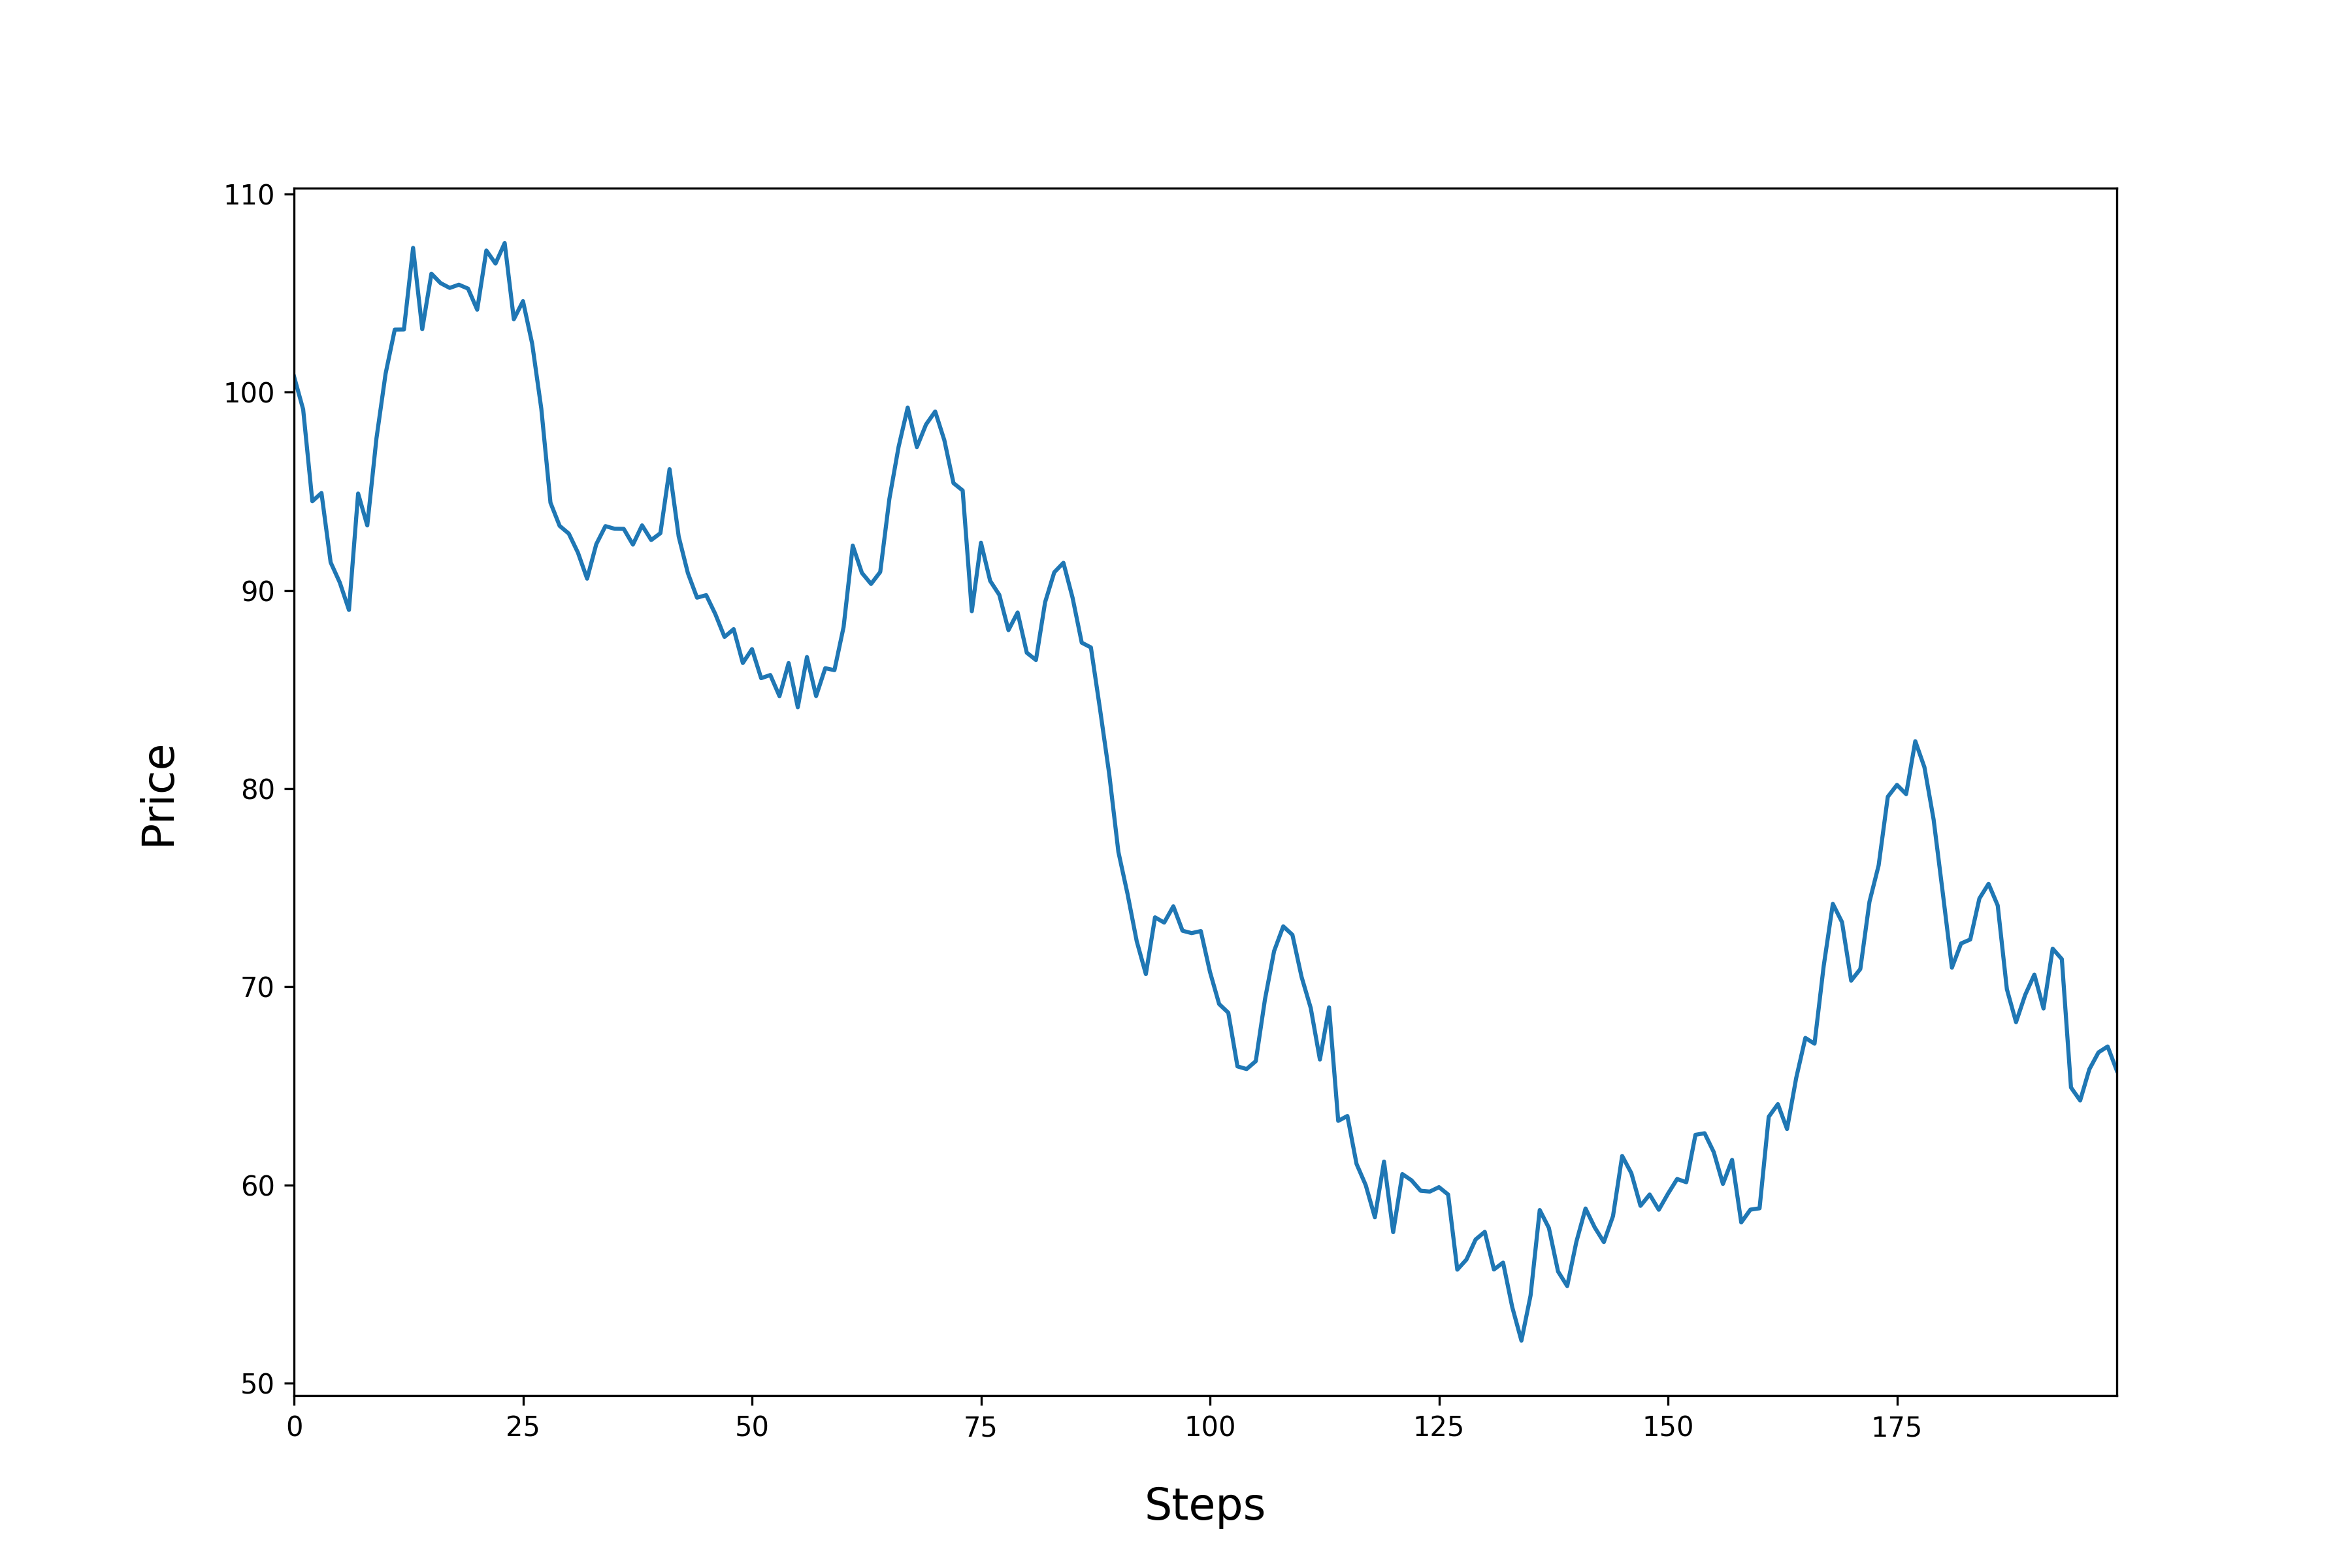
\includegraphics[width=\linewidth]{test.png}
\caption{Third subfigure} \label{fig:c}
\end{subfigure}\hspace*{\fill}
\begin{subfigure}{0.5\textwidth}
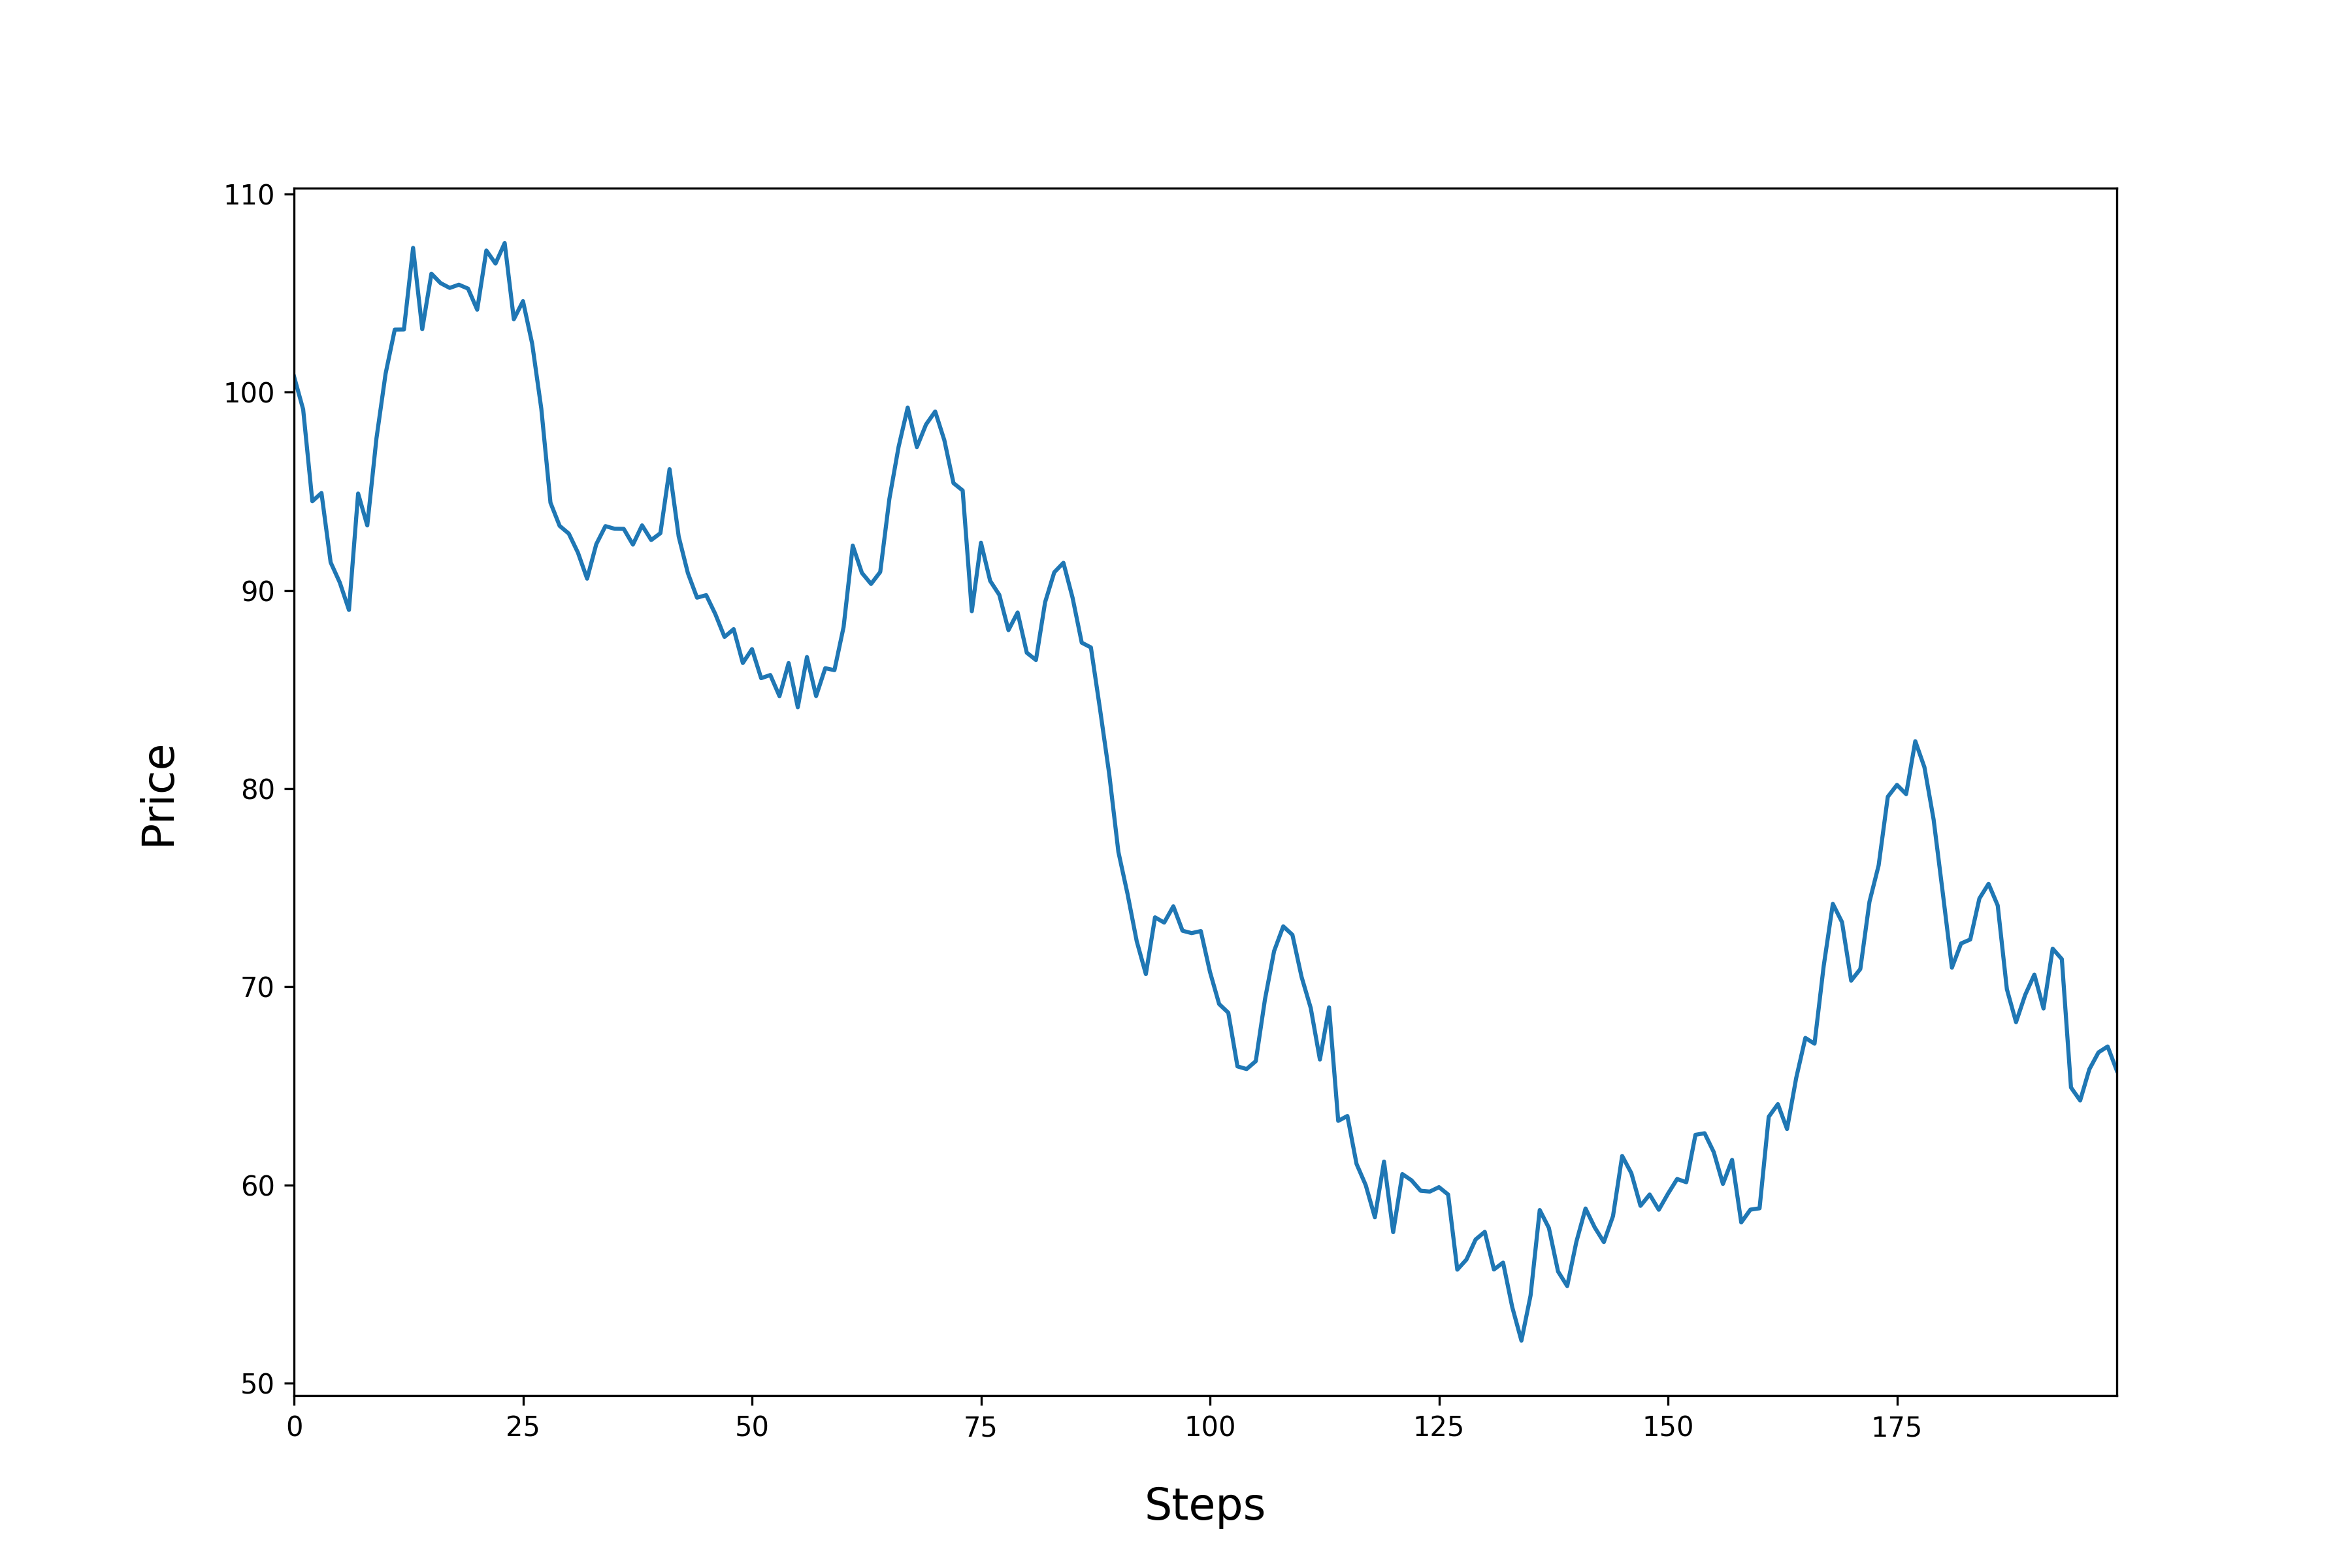
\includegraphics[width=\linewidth]{test.png}
\caption{Fourth subfigure} \label{fig:d}
\end{subfigure}

\medskip
\begin{subfigure}{0.49\textwidth}
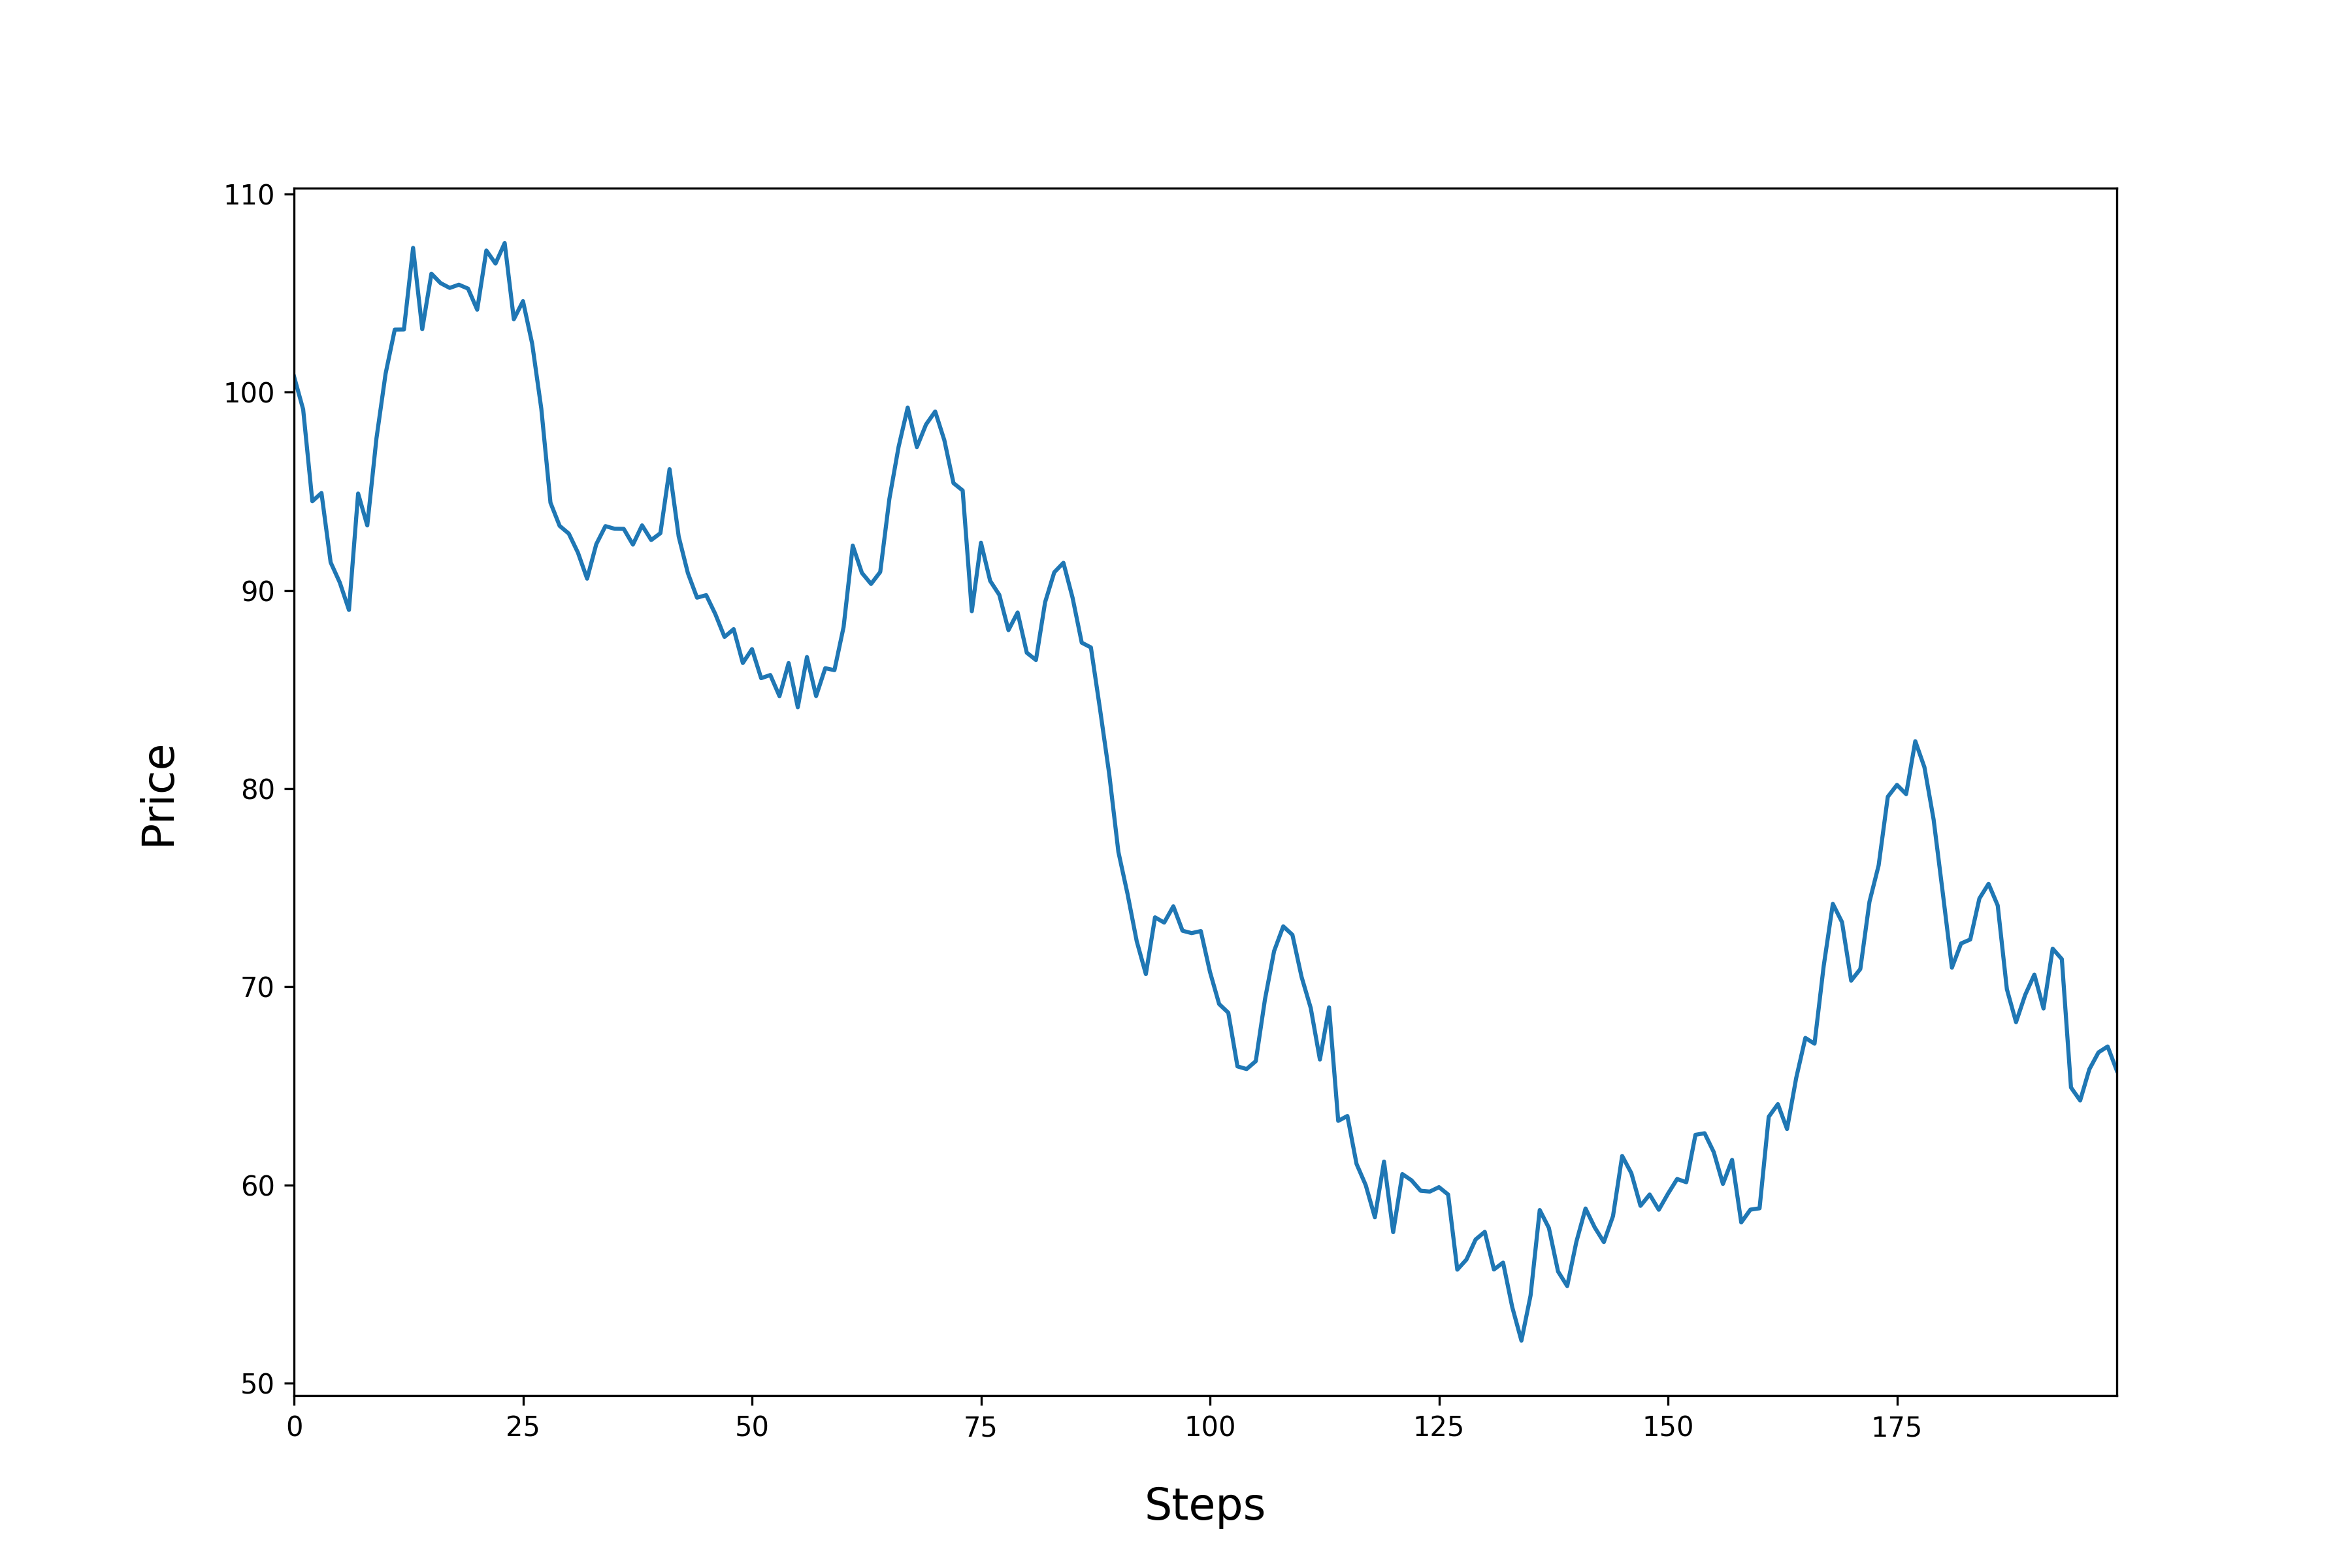
\includegraphics[width=\linewidth]{test.png}
\caption{Fifth subfigure} \label{fig:e}
\end{subfigure}\hspace*{\fill}
\begin{subfigure}{0.49\textwidth}
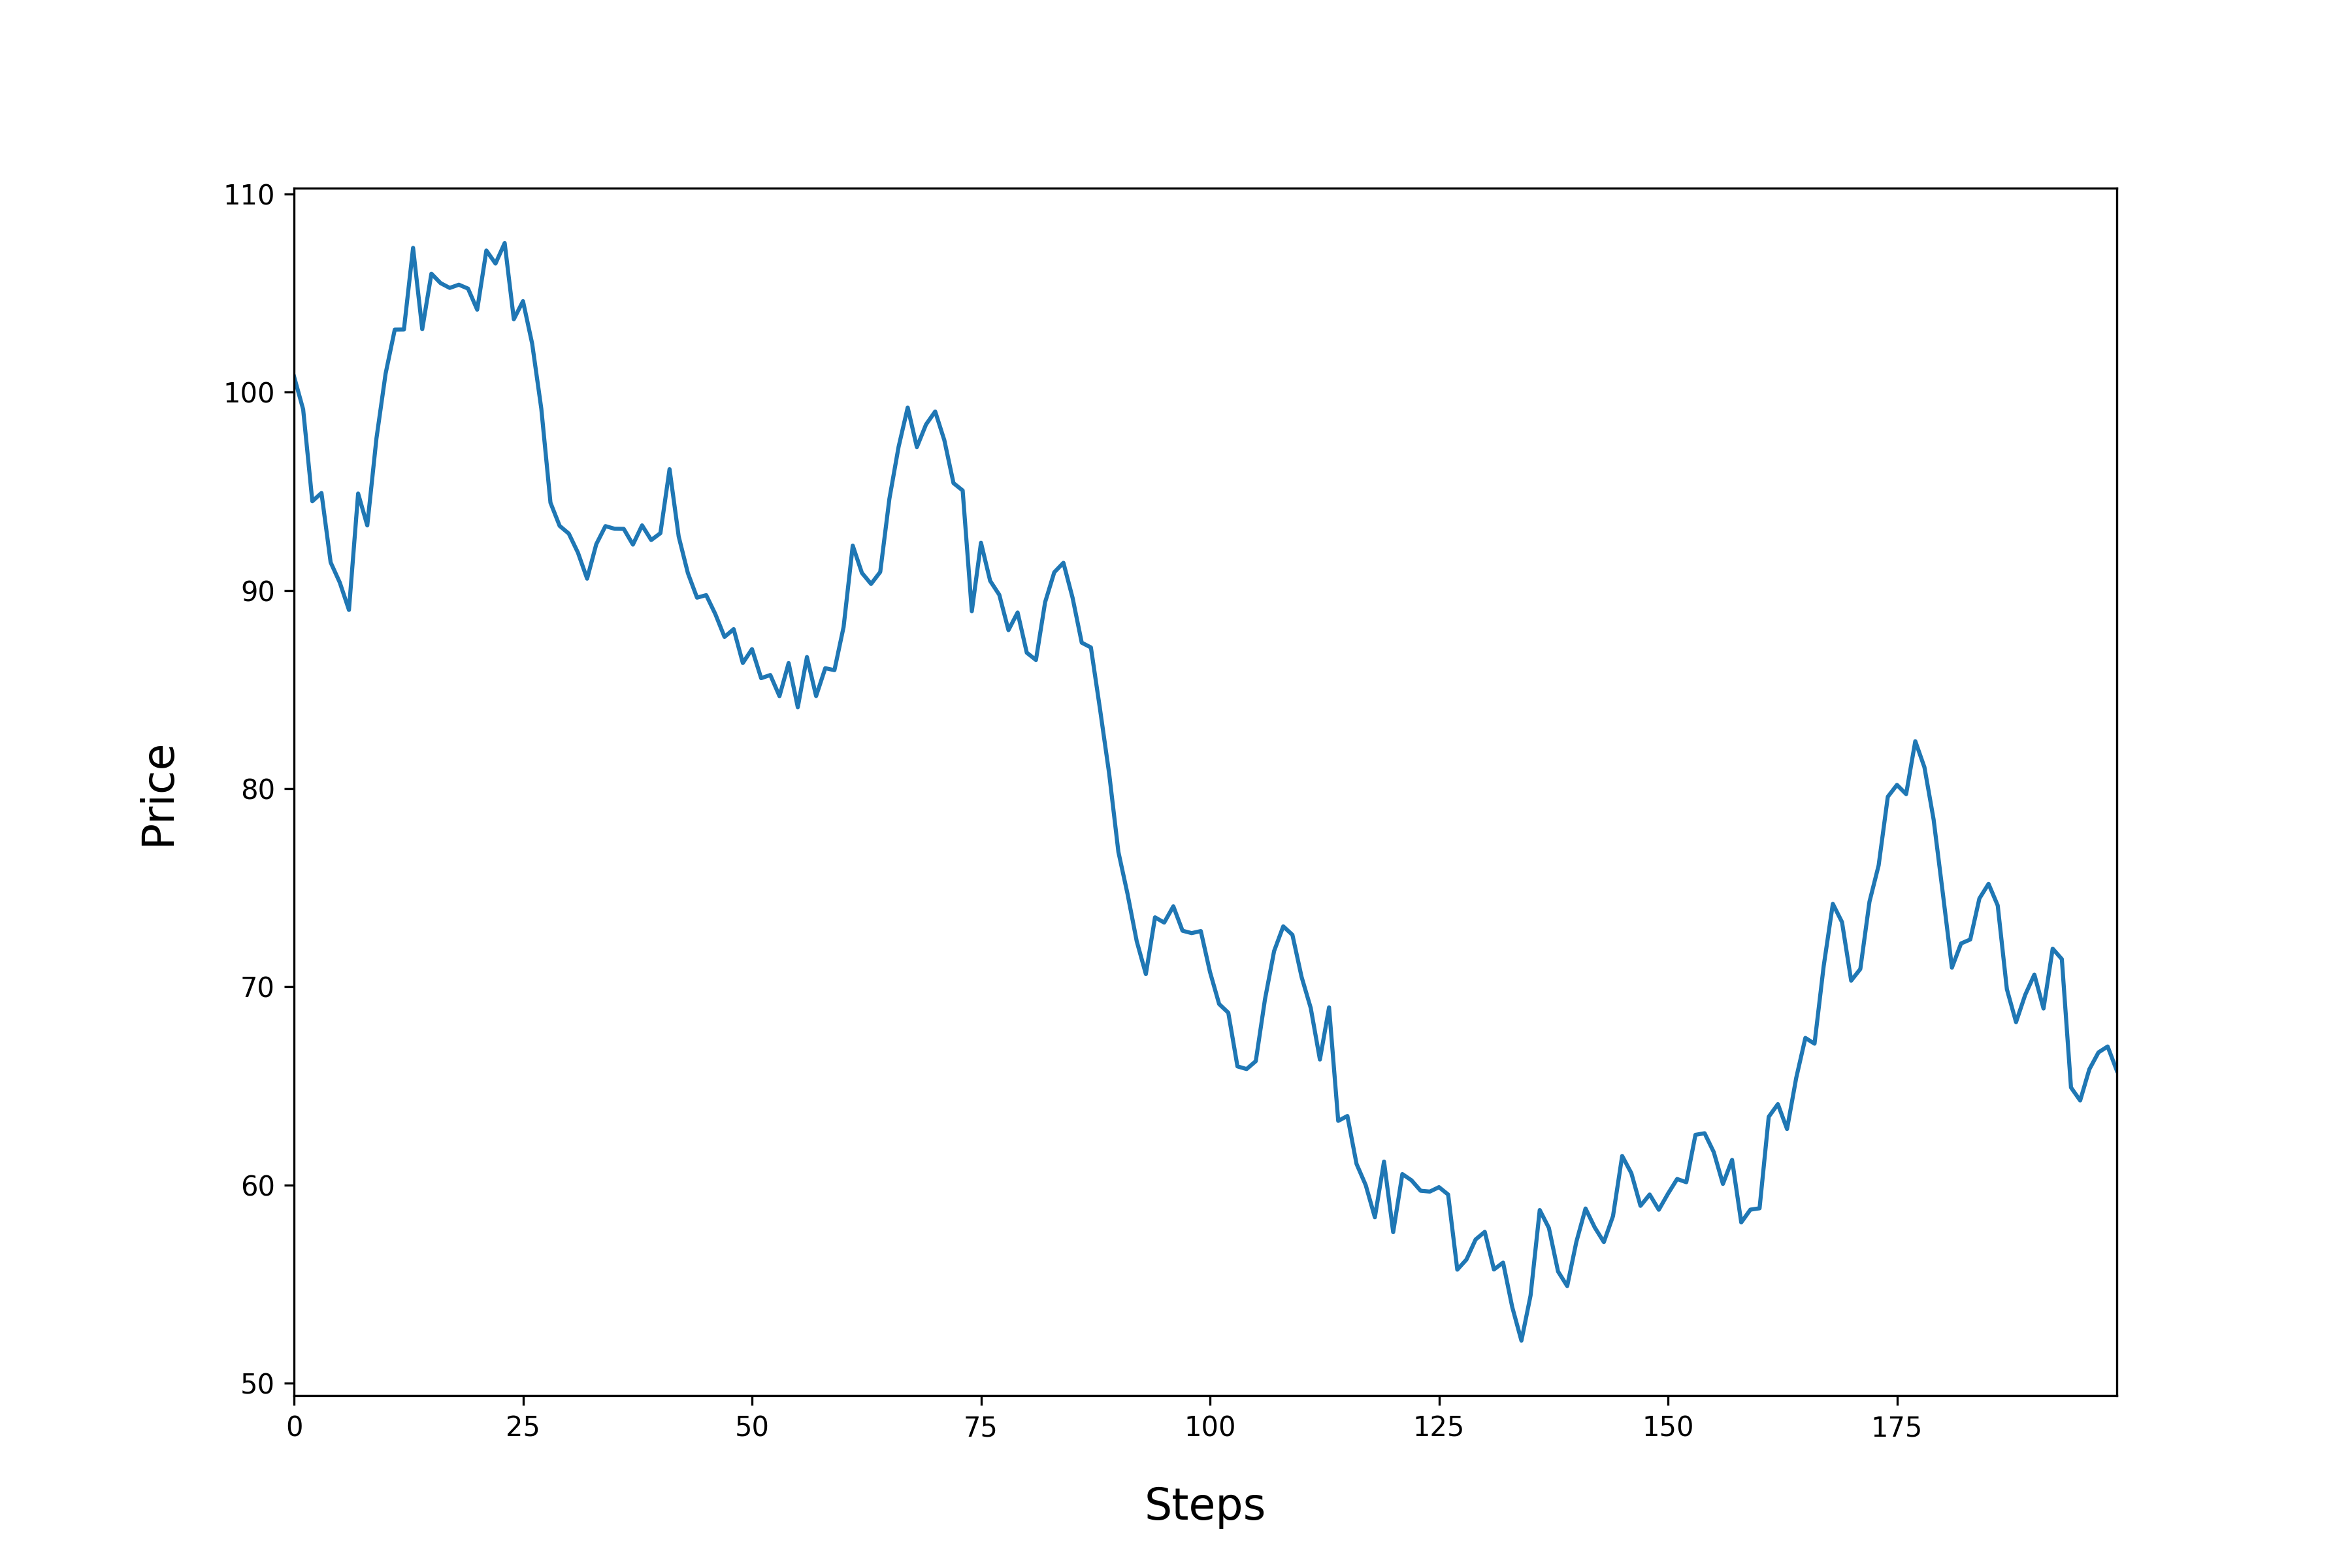
\includegraphics[width=\linewidth]{test.png}
\caption{Sixth subfigure} \label{fig:f}
\end{subfigure}

\caption{My complicated figure} \label{fig:1}
\end{figure}

\section{Conclusion}
\label{sec:conclusion}

\bibliographystyle{unsrt}  

%%% Comment out this section when you \bibliography{references} is enabled.
\begin{thebibliography}{1}

\bibitem{ho1980on}
Thomas Ho and Hans R. Stoll.
\newblock On Dealer Markets Under Competition.
\newblock In {\em The Journal of Finance, Vol. 35, No. 2, Papers and Proceedings Thirty-Eighth Annual Meeting American Finance Association}, pages 259--267. Wiley, 1980.

\bibitem{avellaneda2008high}
Marco Avellaneda and Sasha Stoikov.
\newblock High-frequency trading in a limit order book.
\newblock In {\em Quantitative Finance, Vol. 8, No. 3}, pages 217--224. Routledge, 2008.

\bibitem{guéant2012dealing}
Olivier Guéant, Charles-Albert Lehalle, and Joaquin Fernandez Tapia.
\newblock Dealing with the Inventory Risk. A solution to the market making problem.
\newblock In {\em 	arXiv:1105.3115v5}, 2012.

\bibitem{bouchard2002statistical}
J.-P. Bouchaud, M. Mezard, and M. Potters.
\newblock Statistical properties of stock order books: empirical results and models.
\newblock In {\em arXiv:cond-mat/0203511v2}, 2002.

\bibitem{fushimi2018optimal}
Takahiro Fushimi, Christian González Rojas, and Molly Herman.
\newblock Optimal High-Frequency Market Making.
\newblock 2018.

\bibitem{monti2009impact}
Marco Monti, Laura Martignon, Gerd Gigerenzer, and Nathan Berg.
\newblock The impact of simplicity on financial decision-making.
\newblock In {\em Taatgen, Niels; Van Rijn, Hedderik;: Proceedings of the 31st Annual Conference of the Cognitive Science Society}, pages 1846--1851. Cognitive Science Society, 2009.

\bibitem{wealthfront}
Wealthfront: Financial Planning and Robo-Investing for Millennials.
\newblock \emph{https://www.wealthfront.com/}

\bibitem{betterment}
Betterment.
\newblock \emph{https://www.betterment.com/}

\end{thebibliography}


\end{document}
